\documentclass[
	10pt,								% globale Schriftgröße
	parskip=half-,						% setzt Absatzabstand hoch
	paper=a4,							% Format
	english,ngerman,					% lädt Sprachpakete
	]{scrartcl}							% Dokumentenklasse

% //////////////////// Pakete laden ////////////////////
\usepackage[fleqn]{amsmath}
\usepackage[fleqn]{mathtools}
\usepackage{amssymb}			% mathematische symbole, für \ceckmarks
\usepackage{amsthm}				% für proof
\usepackage{mathrsfs}			% für \mathscr
\usepackage{latexsym}
\usepackage{marvosym}				% für Lightning

\usepackage{fontspec} 			% funktioniert nur mit den neueren Compilern z.B. XeLaTeX
\usepackage{microtype}			% für bessere Worttrennung
\usepackage[ngerman]{babel} 	% Spracheinstellung
\usepackage{lmodern}			% verändert verwendete Schriftart, damit sie weniger pixelig ist

\usepackage{verbatim}
\usepackage{listings}			% Für Quellcode

\usepackage{graphicx}
\usepackage{tabularx}			% für Tabellen mit gleicher Spaltenbreite und automatischen Umbrüchen
\usepackage{fullpage}
\usepackage{multirow}			% für multirow in tabulars
\usepackage{rotate}
\usepackage[cmyk,table]{xcolor} % um Farben zu benutzen, kann mehr als das Paket color
\usepackage[					% Verlinkungen
	colorlinks,					% farbige Schrift, statt farbiger Rahmen
	linktocpage,				% verlinkt im Abb.Verzeichnis Seitenzahl statt Bildunterschrift
	linkcolor=blue				% setzt Farbe der Links auf blau
	]{hyperref}					% nur für digitale Anwendungen, url = "http://www.example.com"
\usepackage{url}				% für Webadressen wie e-mail usw.: "\url{http://www.example.com}"

\usepackage{enumerate}			% für versch. Aufzählungezeichen wie z.B. a)
\usepackage{xspace}				% folgt ein Leerzeichen nach einem \Befehl, wird es nicht verschluckt.
\usepackage{cancel}				% für das Durchstreichen u.a. in Matheformeln mit \cancel
\usepackage{float}              % zum Forcieren der Position von figure-Umgebungen

% zum Zeichnen (u.a. von Graphen)
\usepackage{fp}
\usepackage{tikz}
\usetikzlibrary{tikzmark}			% für \tikzmark{toRemember}
\usetikzlibrary{positioning}	% verbesserte Positionierung der Knoten
\usetikzlibrary{automata}		% für Automaten (GTI)
\usetikzlibrary{arrows}
\usetikzlibrary{shapes}
\usetikzlibrary{decorations.pathmorphing}
\usetikzlibrary{decorations.pathreplacing}
\usetikzlibrary{decorations.shapes}
\usetikzlibrary{decorations.text}

% //////////////////// Syntaxhighlighting ////////////////////
\lstloadlanguages{Python, Haskell, [LaTeX]TeX, Java}
\lstset{
   basicstyle=\footnotesize\ttfamily,	% \scriptsize the size of the fonts that are used for the code
   backgroundcolor = \color{bgcolour},	% legt Farbe der Box fest
   breakatwhitespace=false,	% sets if automatic breaks should only happen at whitespace
   breaklines=true,			% sets automatic line breaking
   captionpos=t,				% sets the caption-position to bottom, t for top
   commentstyle=\color{codeblue}\ttfamily,% comment style
   frame=single,				% adds a frame around the code
   keepspaces=true,			% keeps spaces in text, useful for keeping indentation
							% of code (possibly needs columns=flexible)
   keywordstyle=\bfseries\ttfamily\color{codepurple},% keyword style
   numbers=left,				% where to put the line-numbers;
   							% possible values are (none, left, right)
   numberstyle=\tiny\color{codegreen},	% the style that is used for the line-numbers
   numbersep=5pt,			% how far the line-numbers are from the code
   stepnumber=1,				% nummeriert nur jede i-te Zeile
   showspaces=false,			% show spaces everywhere adding particular underscores;
							% it overrides 'showstringspaces'
   showstringspaces=false,	% underline spaces within strings only
   showtabs=false,			% show tabs within strings adding particular underscores
   flexiblecolumns=false,
   tabsize=1,				% the step between two line-numbers. If 1: each line will be numbered
   stringstyle=\color{orange}\ttfamily,	% string literal style
   numberblanklines=false,				% leere Zeilen werden nicht mitnummeriert
   xleftmargin=1.2em,					% Abstand zum linken Layoutrand
   xrightmargin=0.4em,					% Abstand zum rechten Layoutrand
   aboveskip=2ex, 
}

\lstdefinestyle{py}{
   language=Python,
}
\lstdefinestyle{hs}{
   language=Haskell,
}
\lstdefinestyle{tex}{
	language=[LaTeX]TeX,
	escapeinside={\%*}{*)},     % if you want to add LaTeX within your code
	texcsstyle=*\bfseries\color{blue},% hervorhebung der tex-Schlüsselwörter
	morekeywords={*,$,\{,\},\[,\],lstinputlisting,includegraphics,
	rowcolor,columncolor,listoffigures,lstlistoflistings,
	subsection,subsubsection,textcolor,tableofcontents,colorbox,
	fcolorbox,definecolor,cellcolor,url,linktocpage,subtitle,
	subject,maketitle,usetikzlibrary,node,path,addbibresource,
	printbibliography},% if you want to add more keywords to the set
     numbers=none,
     numbersep=0pt,
     xleftmargin=0.4em,
}

\lstdefinestyle{java}{
	language=Java,
	extendedchars=true,		% lets you use non-ASCII characters;
   						% for 8-bits encodings only, does not work with UTF-8
}

\lstdefinelanguage[x64]{Assembler}     % add a "x64" dialect of Assembler
   [x86masm]{Assembler} % based on the "x86masm" dialect
   % with these extra keywords:
   {morekeywords={CDQE,CQO,CMPSQ,CMPXCHG16B,JRCXZ,LODSQ,MOVSXD, %
                  POPFQ,PUSHFQ,SCASQ,STOSQ,IRETQ,RDTSCP,SWAPGS, %
                  rax,rdx,rcx,rbx,rsi,rdi,rsp,rbp, %
                  r8,r8d,r8w,r8b,r9,r9d,r9w,r9b}
}					% for 8-bits encodings only, does not work with UTF-8

\lstdefinestyle{c}{
	language=c,
	extendedchars=true,		% for 8-bits encodings only, does not work with UTF-8
}

% //////////////////// eigene Kommandos ////////////////////
\newcommand\FU{Freie Universität Berlin\xspace}% benötigt package xspace
\newcommand\gdw{g.\,d.\,w.\xspace}
\newcommand\oBdA{o.\,B.\,d.\,A.\xspace}
\newcommand{\Eu}{\texteuro}
\newcommand\N{\mathbb{N}\xspace}
\newcommand\Q{\mathbb{Q}\xspace}
\newcommand\R{\mathbb{R}\xspace}
\newcommand\Z{\mathbb{Z}\xspace}
\newcommand\ohneNull{\ensuremath{\backslash\lbrace 0\rbrace}}% \{0}
\let\dhALT\dh	% Schreibt Befehl \dh in \dhALT um
\renewcommand\dh{d.\,h.\xspace}	%renew überschreibt command \dh
\newcommand\Bolt{\;\text{\LARGE\raisebox{-0.3em}{\Lightning}\normalsize}\xspace}% Blitz
\newcommand\zz{\ensuremath{\raisebox{+0.25ex}{Z}% zu zeigen
			\kern-0.4em\raisebox{-0.25ex}{Z}%
			\;\xspace}}
\newcommand{\from}{\ensuremath{\colon}}
\newcommand{\floor}[1]{\lfloor{#1}\rfloor}
\newcommand{\ceil}[1]{\lceil{#1}\rceil}
 \renewcommand{\L}{\ensuremath{\mathcal{L}}\xspace}
 \renewcommand{\P}{\ensuremath{\mathcal{P}}\xspace}
 \newcommand{\NL}{\ensuremath{\mathcal{N}\kern-0.2em\mathcal{L}}\xspace}
 \newcommand{\NP}{\ensuremath{\mathcal{NP}}\xspace}

% //////////////////// Mathefunktionen ////////////////////
\DeclareMathOperator{\Landau}{\mathcal{O}}
\DeclareMathOperator{\True}{True}
\DeclareMathOperator{\False}{False}

% //////////////////// eigene Theoreme ////////////////////
\newtheorem{theorem}{Satz}
\newtheorem{corollary}[theorem]{Folgerung}
\newtheorem{lemma}[theorem]{Lemma}
\newtheorem{observation}[theorem]{Beobachtung}
\newtheorem{definition}[theorem]{Definition}
\newtheorem{Literatur}[theorem]{Literatur}
% konfiguriert proof
\makeatletter
\newenvironment{Proof}[1][\proofname]{\par
  \pushQED{\qed}%
  \normalfont \topsep6\p@\@plus6\p@\relax
  \trivlist
  \item[\hskip\labelsep
%         \itshape
        \bfseries
    #1\@addpunct{.}]\ignorespaces
}{%
  \popQED\endtrivlist\@endpefalse
}
\makeatother

% //////////////////// eigene Farben ////////////////////
\let\definecolor=\xdefinecolor
\definecolor{FUgreen}{RGB}{153,204,0}
\definecolor{FUblue}{RGB}{0,51,102}

\definecolor{middlegray}{rgb}{0.5,0.5,0.5}
\definecolor{lightgray}{rgb}{0.8,0.8,0.8}
\definecolor{orange}{rgb}{0.8,0.3,0.3}
\definecolor{azur}{rgb}{0,0.7,1}
\definecolor{yac}{rgb}{0.6,0.6,0.1}
\definecolor{Pink}{rgb}{1,0,0.6}

\definecolor{bgcolour}{rgb}{0.97,0.97,0.97}
\definecolor{codegreen}{rgb}{0,0.6,0}
\definecolor{codegray}{rgb}{0.35,0.35,0.35}
\definecolor{codepurple}{rgb}{0.58,0,0.82}
\definecolor{codeblue}{rgb}{0.4,0.5,1}

% //////////////////// eigene Settings ////////////////////

\textheight = 230mm		% Höhe des Satzspiegels / Layouts
\footskip = 10ex			% Abstand zw. Fußzeile und Grundlinie letzter Textzeile
\parindent 0pt			% verhindert Einrückung der 1. Zeile eines Absatzes
\setkomafont{sectioning}{\rmfamily\bfseries}% setzt Ü-Schriften in Serifen, {disposition}											% bindet Header ein (WICHTIG)
\usepackage{graphicx}
\usepackage{fancyvrb}

\newcommand{\dozent}{Prof. Dr. Agn`es Voisard, Nicolas Lehmann}					% <-- Names des Dozenten eintragen
\newcommand{\tutor}{Nicolas Lehmann}						% <-- Name eurer Tutoriun eintragen
\newcommand{\tutoriumNo}{10}				% <-- Nummer im KVV nachschauen
\newcommand{\projectNo}{6}									% <-- Nummer des Übungszettels
\newcommand{\veranstaltung}{Datenbanksysteme}	% <-- Name der Lehrveranstaltung eintragen
\newcommand{\semester}{SoSe 2017}						% <-- z.B. SoSe 17, WiSe 17/18
\newcommand{\studenten}{Boyan Hristov, Julian Habib}			% <-- Hier eure Namen eintragen
% /////////////////////// BEGIN DOKUMENT /////////////////////////

\begin{document}

% /////////////////////// BEGIN TITLEPAGE /////////////////////////
\begin{titlepage}
	\subject{\dozent}
	\title{\veranstaltung, \semester}
	\subtitle{\Large Übungsblatt \projectNo\\ \large\vspace{1ex} TutorIn: \tutor\\ Tutorium \tutoriumNo}
	\author{\studenten}
	\date{\normalsize \today}
\end{titlepage}

\maketitle								% Erstellt das Titelblatt
\vspace*{-10cm}							% rückt Logo an den oberen Seitenrand
\makebox[\dimexpr\textwidth+1cm][r]{	%rechtsbündig und geht rechts 1cm über Layout hinaus
	
\includegraphics[width=0.4\textwidth]{src/fu_logo} % fügt FU-Logo ein
}
% /////////////////////// END TITLEPAGE /////////////////////////

\vspace{7cm}							% Abstand
\rule{\linewidth}{0.8pt}				% horizontale Linie										% erstellt die Titelseite

Link zum Git Repository: \url{https://github.com/BoyanH/Freie-Universitaet-Berlin/tree/master/Datenbanksysteme/Solutions/homework\projectNo}

% /////////////////////// Aufgabe 1 /////////////////////////

\section*{1. Aufgabe}

\begin{enumerate}

\item[a)]
z.z.: $R_1$ ist in 1NF \\
$R_1$ ist in 1NF $\Leftrightarrow$ alle Attribute sind atomar. \\ \\
$R_1(A,B,C,D) \subseteq A \times B \times C \times D \Rightarrow $ A,B,C,D sind atomar.

Alle Attributen in $R_1$ haben atomäre Domäne, sind also keine Relationen. Z.B. alle Einträge haben für den Attribut A die Werte $a_1, a_2, a_3$ und keine Werte wie z.B. $(a_1, a_2)$.

$\hfill \Box$

\item[b)]
z.z.: $R_1$ ist nicht in 2NF \\ \\
$R_1$ ist in 2NF $\Leftrightarrow$  $R_1$ ist in 1NF und $\forall (X \rightarrow A) \in F_{+} | A \not\in X: X \not\subset $ Superschlüssel $\lor A \subseteq$ Schlüssel.

Beweis durch Gegenbeispiel:

\begin{align*}
    FD(R_1) = \{ & \\
    & A \rightarrow B \\
    & A \rightarrow C \\
    & D \rightarrow C \\
    & BD \rightarrow A \\
    \} & \\
    \Rightarrow & \text{ AD und BD sind Superschlüssel und auch beide Kandidatschlüsseln.} \\
    & \text{Primäre Attributen sind A, B und D. }
\end{align*}

Da C kein Primärattribut ist, von A abhängig ist und da A eine Untermenge eines Schlüssels ist (AD), ist $R_1$ nicht in 2NF.

$\hfill \Box$

\item[c)]
z.z.: $R_2$  ist in 3NF \\
$R_2$  ist in 3NF $\Leftrightarrow \forall FD(X \rightarrow A):$ X ist Superschlüssel von R oder A ist Primärattribut von R

Direkter Beweis: 

\begin{align*}
    FD(R_2) = \{ & \\
    & E \rightarrow F \\
    & E \rightarrow G \\
    & FG \rightarrow E \\
    \} & \\
    \Rightarrow & \text{ E und FG sind Superschlüssel, Primärattributen sind E, F und G. }
\end{align*}

In den ersten zwei funktionalen Abhängigkeiten ist die linke Seite ein Superschlüssel, in der 3. Abhängigkeit ist die rechte Seite ein Primärattribut.
$\Rightarrow R_2$ ist in 3NF.

$\hfill \Box$

\item[d)]

z.z: $R_2$ ist in BCNF \\
$R_2$ ist in BCNF $\Leftrightarrow \forall X \rightarrow A \in F_{+}:$ X ist Superschlüssel.

Direkter Beweis: 

\begin{align*}
    FD^{+}(R_2) = \{ & \\
    & E \rightarrow F \\
    & E \rightarrow G \\
    & E \rightarrow FG \\
    & FG \rightarrow E \\
    \} &
\end{align*}

Da wir schon aus c) kennen, dass E und FG Superschlüssel sind und da diese alle mögliche linke Seiten von einer funktionalen Abhängigkeit sind, ist $R_2$ in Boyce-Codd Normalform (BCNF).

$\hfill \Box$

\end{enumerate}

\section*{2. Aufgabe}

\begin{enumerate}

\item[a)]
Mit dem Algorithmus aus der Vorlesung für "Well-behaved 3NF Decomposition"

\begin{align*}
    FD(R_3) = \{ & \\
    & H \rightarrow JK \\
    & I \rightarrow HJ \\
    & K \rightarrow L \\
    \} &
\end{align*}

\begin{enumerate}
\item[1.] For each FD (X $\rightarrow$ A) in F 
create a relation with schema (XA). \\

\begin{align*}
    (HJK), (IHJ), (KL)
\end{align*}

\item[2.] If none of the keys appears in one of the schemas of 1
then add a relation with schema Y, with Y a key. \\

$\Rightarrow$ fertig, da H ein Schlüssel ist und in (HJK) vorhanden ist.

\item[3.] If for relations created in 1. there exists a relation R1 whose
schema is included in the schema of another relation, then remove
R1. \\

Alles ist in Ordnung, die Attributen von keinem Schema sind eine Untermenge von den Attributen eines anderen Schemas.

\item[4.] Replace relations (X A1), ..., (X Ak)
with a single relation (X A1 ... Ak).

\begin{align*}
     & (HJK) \land (IHJ) \Rightarrow (HJIK)
\end{align*}

\end{enumerate}



Gute Zerlegung: $R_{31}(H,J,I,K)$ und $R_{32}(K,L)$

\item[b)]

\begin{align*}
    & R_{31} \cap R_{32} \equiv K \\
    & R_{31} - R_{32} \equiv HJI
    & R_{32} - R_{31} \equiv L \\ \\
    & R_{31} \cap R_{32} \rightarrow KL  \text{ (wegen K $\rightarrow$ L) }
        \rightarrow L \equiv R_{31} - R_{32} \\
    \Rightarrow & \text{ Unsere Zerlegung ist verlustlos} 
\end{align*}

\item[c)]

\begin{align*}
    & FD(R_{31}) = \{ H \rightarrow JK, I \rightarrow HJ \} \\
    & FD(R_{32}) = \{ K \rightarrow L \} \\
    & FD(R_{31}) \cup FD(R_{32}) \equiv \{ H \rightarrow JK, I \rightarrow HJ, K \rightarrow L \} \equiv FD(R_3) \\
    \Rightarrow & \text{ Unsere Zerlegung ist abhängigkeitserhaltend}
\end{align*}

\item[d)]
Da wir dieses Algorithmus benutzt haben, ist jede davon entstandene Relation in 3NF. Wegen b), c) und d) ist die Zerlegung gut. Für $R_{32}$ sind H und I Schlüssel und an alle funktionalen Abhängigkeiten auf der linken Seite vorhanden, deswegen ist $R_{32}$ in 3NF. $R_{32}$ hat nur eine funktionale Abhängigket und nur 2 Attributen, ist deswegen trivialerweise in 3NF.


\end{enumerate}

\section*{3. Aufgabe}

\begin{enumerate}

    \item[a)]
    Aus jedem Item kann man durch eine Hash-Funktion ein Hash erzeugen durch mathematische Umformungen aus allen Suchschlüssel. Mehrere Items werden in dem selben Bucket gespeichert (nacheinandere folgende Blöcke im Speicher) wenn die Hashfunktion das gleiche Hash aus ihren Suchschlüssel erzeugt. Danach, beim Suchen von Lösch / Einfüge / Lese Position müssen alle Einträge in dem entsprechenden Bucket nach einander geprüft werden. Deswegen erzeugen gute Hashfunktione randomisierte Hashes, damit es ungefähr genau so viele Items pro Bucket gibt.

    \item[b)]
    In einem Dense-Index gibt es Indizes für alle Suchschlüsselwerte. Z.b. wenn das Attribut A ein Primärindex ist, gibt es für alle mögliche Werte von A ein Index, die Einträge mit dem gleichen Wert von A stehen nach einander im Speicher.

    Der Sparse-Index hat nur für gewählte Werte von den Suchschlüssel Indizes. Dabei müssen aber immer die Einträge im Speicher nach dem Primärindex sortiert werden. Damit sucht man nach dem Index des alphabetisch größten kleineren Wert und muss dann alle weitere Einträge durchsuchen, um den Item zu finden. Dabei haben wir viel speicher für den Index gespart, die Suchzeiten haben sich aber vergrößert. Ein gutes Balance zwischen den beiden ist zu finden.

    \item[c)]
    Ein Multilevel-Index ist ein Index, wo das unterste Niveau ein Dense-Index ist und darüber noch n Stufen von Sparse-Index existieren. So kann man viel Schneller suchen ($log_2(n)$, da es so viele Schritten vom Wurzel zu den Blätter in einem balancierten Baum mit n Blätter gibt). Die Blätter eines $B^{+}$ Baums sind die äußeren Indizes und die restliche Knoten die innere Indizes. Diese Struktur darf man aber nur dann verwenden, wenn die Suchschlüssel sortierbar sind, da man sonst kein $B^{+}$ oder überhaupt kein Suchbaum konstruieren kann.

    \item[d)]
    "Fixed Length Records" \\
    Sei 3 die Länge eines Records \\ \\
    \begin{tabular}{ l | l | l | l |}
    \hline
    \#record & Film Name & Actor's Name & Actor's Address \\ \hline
    0 & Fremde Gewässer & Thomas Depp & Paris \\ \hline
    1 & Fremde Gewässer & Linda Cruz & Los Angeles \\ \hline
    2 & Furious Sixteen & Martin Diesel & Detroid \\ \hline
    3 & Furious Sixteen & Grünther Walker & New York
    \end{tabular}

    "Variable Length Records" \\ \\
    \begin{tabular}{| l | l | l | l | l | l | l |}
    \hline
    \#record & Film Name & Actor's Name & Actor's Address & Actors's Name & ... & ... \\ \hline
    0 & Fremde Gewässer & Thomas Depp & Paris & Linda Cruz & Los Angeles & $\perp$ \\ \hline
    1 & Furious Sixteen & Martin Diesel & Detroid & Grünther Walker & New York & $\perp$ \\ \hline
    \end{tabular}

    Mit Hilfe von Pointer \\

    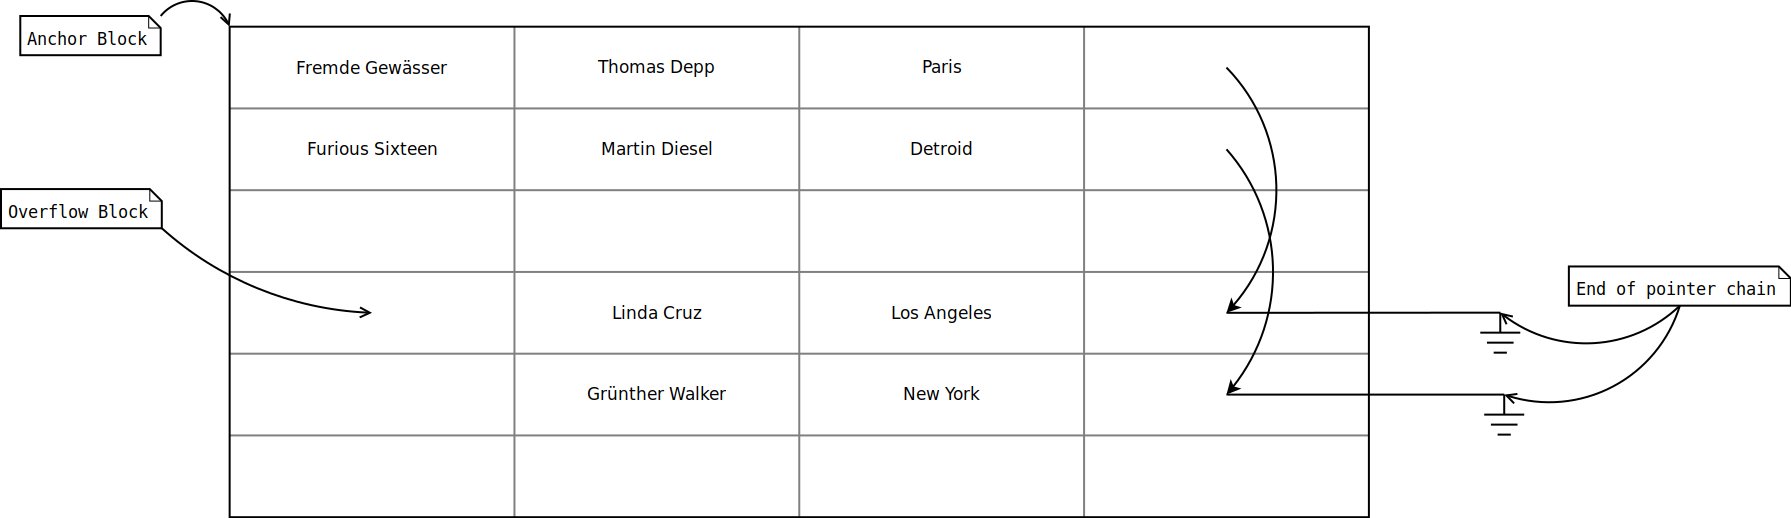
\includegraphics[width=\textwidth]{pointerRepresentation.png}

\end{enumerate}

\section*{Aufgabe 3.}

\begin{enumerate}

\item[a)]

\includegraphics[width=\textwidth]{./images/a1.jpg}
\includegraphics[width=\textwidth]{./images/a2.jpg}

\item[b)]

\includegraphics[width=\textwidth]{./images/b1.jpg}

\item[c)]

\includegraphics[width=\textwidth]{./images/c1.jpg}
\includegraphics[width=\textwidth]{./images/c2.jpg}

\end{enumerate}

% /////////////////////// END DOKUMENT /////////////////////////
\end{document}
